\documentclass[12pt,a4paper,austrian]{article}
\usepackage{graphicx}
\usepackage[austrian, english]{babel}
\usepackage[utf8]{inputenc}
%\usepackage{listings}
\usepackage{multirow}
\usepackage{epstopdf}
\usepackage{amsmath}
\usepackage{amssymb} % fuer Mengen \N, Q, C, R
\graphicspath{{./fig/}}


%% Satzspiegel
\setlength{\hoffset}{-1in} \setlength{\textwidth}{18cm}
\setlength{\oddsidemargin}{1.5cm}
\setlength{\evensidemargin}{1.5cm}
\setlength{\marginparsep}{0.7em}
\setlength{\marginparwidth}{0.5cm}

\setlength{\voffset}{-1.9in}
\setlength{\headheight}{12pt}
\setlength{\topmargin}{2.6cm}
   \addtolength{\topmargin}{-\headheight}
\setlength{\headsep}{3.5cm}
   \addtolength{\headsep}{-\topmargin}
   \addtolength{\headsep}{-\headheight}
\setlength{\textheight}{27cm}

%% How should floats be treated?
\setlength{\floatsep}{12 pt plus 0 pt minus 8 pt}
\setlength{\textfloatsep}{12 pt plus 0pt minus 8 pt}
\setlength{\intextsep}{12 pt plus 0pt minus 8 pt}

\tolerance2000
\emergencystretch20pt

%% Text appearence
% English text
\newcommand{\eg}[1]%
  {\selectlanguage{english}\textit{#1}\selectlanguage{austrian}}

\newcommand{\filename}[1]
  {\begin{small}\texttt{#1}\end{small}}

\newcommand\IFT{\unitlength1mm\begin{picture}(10,2) \put (1,1)
{\circle{1.7}} \put(2,1){\line(1,0){5}} \put(8,1)
{\circle*{1.7}}\end{picture}}
\newcommand\FT{\unitlength1mm\begin{picture}(10,2) \put (1,1)
{\circle*{1.7}} \put(2,1){\line(1,0){5}} \put(8,1)
{\circle{1.7}}\end{picture}}

% A box for multiple choice problems
\newcommand{\choicebox}{\fbox{\rule{0pt}{0.5ex}\rule{0.5ex}{0pt}}}

\newenvironment{wahrfalsch}%
  {\bigskip\par\noindent\makebox[1cm][c]{richtig}\hspace{3mm}\makebox[1cm][c]{falsch}
   \begin{list}%
   {\makebox[1cm][c]{\choicebox}\hspace{3mm}\makebox[1cm][c]{\choicebox}}%
   {\setlength{\labelwidth}{2.31 cm}\setlength{\labelsep}{3mm}
    \setlength{\leftmargin}{2.61 cm}\setlength{\listparindent}{0pt}
    \setlength{\itemindent}{0pt}}%
  }
  {\end{list}}

\newcounter{theaufgabe}\setcounter{theaufgabe}{1}
\newenvironment{exercise}[1]%
  {\bigskip\par\noindent\begin{nopagebreak}
   \textsf{\textbf{Exercise\thinspace\arabic{theaufgabe}}}\quad
      \textsf{\textit{#1}}\\*[1ex]%
\stepcounter{theaufgabe}\hspace{2ex}\end{nopagebreak}}
  {\par\pagebreak[2]}

% Innerhalb der Aufgaben erfolgt die weitere Unterteilung mittels einer
% enumerate Umgebung, die allerdings a), b),... zaehlen soll.
\renewcommand{\labelenumi}{\alph{enumi})}
\renewcommand{\labelenumii}{\arabic{enumii})}

% A box to tick for everything which has to done
\newcommand{\abgabe}{\marginpar{$\Box$}}
% Margin paragraphs on the left side
\reversemarginpar

% Language for listings
%\lstset{language=Vhdl,
%  basicstyle=\small\tt,
 % keywordstyle=\tt\bf,
 % commentstyle=\sl}

% No indention
\setlength{\parindent}{0.0cm}
% Don't number sections
\setcounter{secnumdepth}{0}


%% Beginning of the text

\begin{document}
\selectlanguage{english}
\pagestyle{plain}


%===  This is the header section ============================================================
\thispagestyle{empty}
\noindent
\begin{minipage}[b][4cm]{1.0\textwidth}
\begin{center}
\begin{bf}
\begin{large} Digital Signal Processing SS 2024 -- 1.~Assignment\end{large} \\
\vspace{0.3cm}
\begin{Large} Analogue Signals and Systems  \end{Large} \\
\vspace{0.3cm}
\end{bf}
\begin{large}
Group 22\\
Julian Feichtinger, K12015812\\
Wolfram Laube, \textless Matrikelnummer \textgreater\\
\end{large}
\end{center}
\end{minipage}

\noindent \rule[0.8em]{\textwidth}{0.12mm}\\[-0.5em]
%=======================================================================================

\begin{exercise}{}
These complex numbers are given:
\begin{align*}
    c_1 = -5 + j3 \\
    c_2 = \frac{\sqrt{2}}{2} \exp^{-j\frac{3\pi}{4}}\\
    c_3 = \frac{1}{\sqrt{2}} + j\frac{1}{\sqrt{2}} = \exp^{j\frac{3}{4}}
\end{align*}

Converting $c_2 = z_2 \exp^{j\varphi_2}$ from polar to cartesian:
\begin{align*}
    a_2 = z_2 \cos \varphi_2 = \frac{\sqrt{2}}{2} \cos\left(-\frac{3\pi}{4}\right) = \frac{\sqrt{2}}{2} \left(-\frac{1}{\sqrt{2}}\right) = -\frac{1}{2} \\
    b_2 = z_2 \sin \varphi_2 = \frac{\sqrt{2}}{2} \sin\left(-\frac{3\pi}{4}\right) = \frac{\sqrt{2}}{2} \left(-\frac{1}{\sqrt{2}}\right) = -\frac{1}{2} \\
    c_2 = a_2 + jb_2 = -\frac{1}{2} - j\frac{1}{2}
\end{align*}

\begin{enumerate}
\item [1.1]
\begin{align*}
    c_4 = c_1 + c_2 = -5 + j3 - \frac{1}{2} - j\frac{1}{2} = - \frac{11}{2} + \frac{j5}{2}
\end{align*}

\item [1.2]
\begin{align*}
    c_5 = c_1 \cdot c_2  = \left(-5 + j3\right) \left(-\frac{1}{2} - j\frac{1}{2}\right) = \frac{5}{2} + j\frac{5}{2} - j\frac{3}{2} - j^2\frac{3}{2} = 4 + j
\end{align*}

\item [1.3]
\begin{align*}
    c_6 = \left|c_3\right|^2 = \left|\frac{1}{\sqrt{2}} + j\frac{1}{\sqrt{2}}\right|^2 = \frac{1}{2} + \frac{1}{2} = 1
\end{align*}

\item [1.4]
\begin{align*}
    c_7 = \arg c_3 = \varphi_3 = \sqrt{\left(\frac{1}{\sqrt{2}}\right)^2 + \left(\frac{1}{\sqrt{2}}\right)^2} = \sqrt{\frac{1}{2} + \frac{1}{2}} = \sqrt{1} = 1
\end{align*}

\item [1.5]
\begin{align*}
    c_8 = \frac{c_1}{c_2} = \frac{c_1}{c_2} \cdot \frac{c_2^*}{c_2^*} = \frac{c_1 c_2^*}{a_2^2 + b_2^2} = \frac{\left(-5 + j3\right) + \left(-\frac{1}{2} - j\frac{1}{2}\right)}{\left(-\frac{1}{2}\right)^2 + \left(-\frac{1}{2}\right)^2} = \frac{\frac{5}{2} + j\frac{5}{2} - j\frac{3}{2} - j^2\frac{3}{2}}{\frac{1}{2}} = 5 + j2 + 3 = 8 + j2
\end{align*}

\item [1.6]
\begin{align*}
    c_9 = c_1 \cdot c_1^* = (-5 + j3) (-5 - j3) = 25 + j15 - j15 - j^2 9 = 25 + 9 = 34
\end{align*}

\end{enumerate}
\end{exercise}



\begin{exercise}{}
Consider the cosine wave given by $x(t) = \hat{X} \cos(2\pi f_0 t)$. We know Eulers formula is given by $\cos x = \frac{e^{jx} + e^{-jx}}{2}$. Then use Eulers formula to express the cosine in the time domain as sum of complex exponentials:
\begin{align*}
    x(t) = \hat{X} \cos(2\pi f_0 t) = \frac{\hat{X}}{2} \left(\exp^{j2\pi f_0 t} + \exp^{-j2\pi f_0 t}\right) = \frac{1}{2} \left(\hat{X}\exp^{j2\pi f_0 t}\right) + \frac{1}{2} \left(\hat{X}\exp^{j2\pi (-f_0) t}\right)
\end{align*}

Applying the Fourier transform (given by $\hat{X}\exp^{j2\pi f_0 t} \rightarrow \hat{X}\delta(f - f_0)$) of a complex exponential function results in:
\begin{align*}
     \frac{1}{2} \left(\hat{X}\delta(f - f_0)\right) + \frac{1}{2} \left(\hat{X}\delta(f - (-f_0))\right) = \frac{\hat{X}}{2} \delta(f - f_0) + \frac{\hat{X}}{2} \delta(f + f_0) = X(f)
\end{align*}


TO DO: Add a diagram of  in the report (draw the real and the imaginary part of in the same diagram).
\end{exercise}








\newpage
% ALLES DARUNTER IST DAS TEMPLATE

\begin{exercise}{}
Eventuell eine allgemeine Erklärung zu dieser Aufgabe (falls notwendig)
\begin{enumerate}
\item [a)]
Anmerkung: Dies sei eine analytische Aufgabe. \\ \\
Hier soll gezeigt werden, dass das zeitdiskrete System
\[
y[n] = x[n] + u[n-3] x[n-1].
\]
linear ist. Dazu wurden folgende Berechnungen durchgeführt:\\
%
\begin{align*}
y_a[n] &= f\left(\underbrace{\alpha x_1[n] + \beta x_2[n]}_{\text{wird in Gleichung für x eingesetzt}}\right)\\ \\
       &= \alpha\,x_1[n] + \beta\,x_2[n] + u[n-3] (\alpha\,x_1[n-1] + \beta\,x_2[n-1])\\ \\
       &= \alpha\,x_1[n] + \beta\,x_2[n] + u[n-3] \alpha\,x_1[n-1] + u[n-3]  \beta\,x_2[n-1] \\ \\
y_b[n] &= \alpha\,f(x_1[n]) + \beta f(x_2[n])\\ \\
       &= \alpha (x_1[n] + u[n-3] x_1[n-1]) + \beta (x_2[n] + u[n-3] x_2[n-1])     \\ \\
       &= \alpha x_1[n] + \alpha u[n-3] x_1[n-1] + \beta x_2[n] + \beta u[n-3] x_2[n-1] \\ \\
       y_a[n] &= y_b[n] \rightarrow \text{linear}
\end{align*}
%
\item [b)]
Anmerkung: In dieser Aufgabe sei eine Funktion zu implementieren. \\ \\
Die Lösung dieses Beispiels finden Sie in \texttt{xxx.m}. Hier können auch eventuelle Probleme geschildert werden (falls etwas nicht ganz funktioniert). Gerne können hier auch Ergebnisse präsentiert werden, welche zeigen, dass die Implementierung korrekt ist (z.B. Diagramme, ...).

\item [c)]
Anmerkung: In dieser Aufgabe seien diverse Plots zu veranschaulichen. \\ \\
Figure~\ref{fig:Testpicture} zeigt ... \\
Diskutieren Sie hier unbedingt, was das Bild zeigt bzw. ob es den Erwartungen entspricht oder nicht. Achten Sie auf eine sinnvolle Darstellung! Wenn in einem Plot nichts erkennbar ist, können auch keine Punkte vergeben werden. Vergessen Sie außerdem nie auf eine korrekte Achsenbeschriftung!
\begin{figure}[!ht]
	\centering
	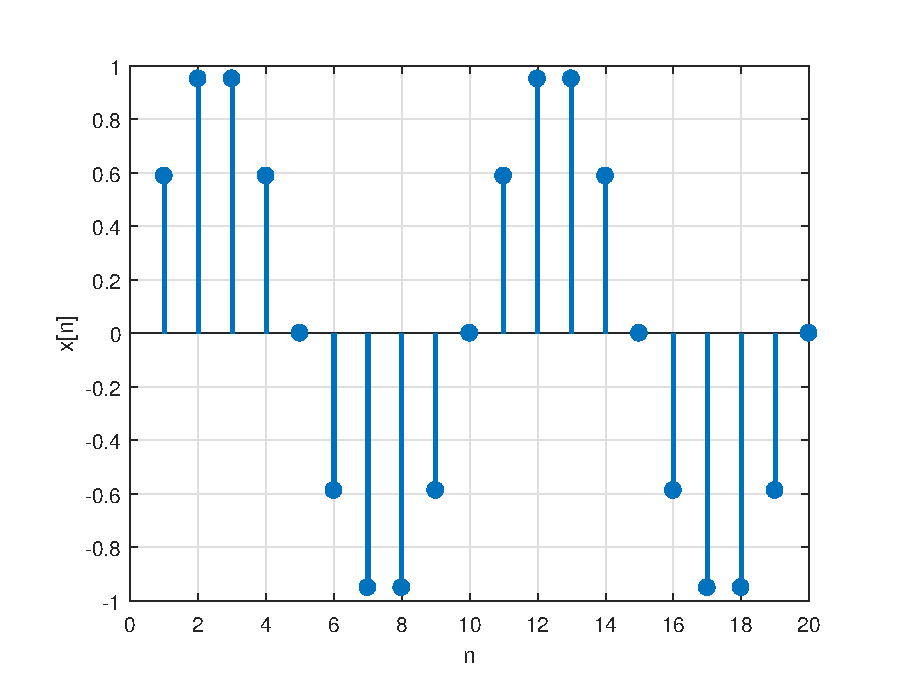
\includegraphics[width=18cm]{Testpicture.eps}
	\vspace{-0.3cm}
	\caption{Das ist ein Testbild im eps Format.}
	\label{fig:Testpicture}
	\vspace{-0.1cm}
\end{figure}

\end{enumerate}
\end{exercise}

\begin{exercise}{}
Erklärung der Aufgabe
\begin{enumerate}
\item [a)]
Teilaufgabe a)

\item [b)]
Teilaufgabe b)


\item [c)]
Teilaufgabe c)

\end{enumerate}
\end{exercise}



\end{document}
